% !TeX program = lualatex
% !TeX root = luaking.tex
% !TeX encoding = UTF-8
% !TeX spellcheck = cs_CZ
%---------------------------------------------------------------------------------------------------
% file fyz3ch01.tex
\graphicspath{{../src/FYZ/img/}}
%---------------------------------------------------------------------------------------------------
%====================Kapitola: Elektrostatika ======================================================
\setchaptertoc
\chapter{Elektrostatika}\label{fyz:IIIchapI}   
  \section{Coulombův zákon}\label{fyz:IIIchapIsecII}
    Při kvantitativním popisu silového působení mezi makroskopickými nabitými tělesy je výhodné v
    prvním přiblížení abstrahovat od způsobu rozložení náboje v objemu tělesa. Můžeme zavést pojem
    \textbf{bodového náboje}, který je analogický pojmu hmotného bodu v mechanice. Za bodový náboj
    můžeme tedy považovat nabité těleso, jehož rozměry jsou zanedbatelně malé ve srovnání se
    vzdálenostmi, na nichž silové působení uvažujeme. Dvojice bodových nábojů o velikostech,
    \(Q_1\), \(Q_1\), které jsou umístěny ve vakuu v bodech o polohových vektorech \(\vec{r}_1\),
    \(\vec{r}_2\) a které jsou nehybné v dané inerciální soustavě souřadnic (obr. \ref{fyz:fig0342}),
    tvoří nejjednodušší makroskopickou soustavu, na níž je možné silové působení mezi náboji
    studovat. Experimenty tohoto druhu provedl r. 1785 \emph{Ch. A. Coulomb} s použitím
    \emph{torzních vah}, které představují jeden z nejcitlivějších fyzikálních přístrojů. 

    \begin{figure}[ht!]  %\ref{fyz:fig0342}
      \centering
      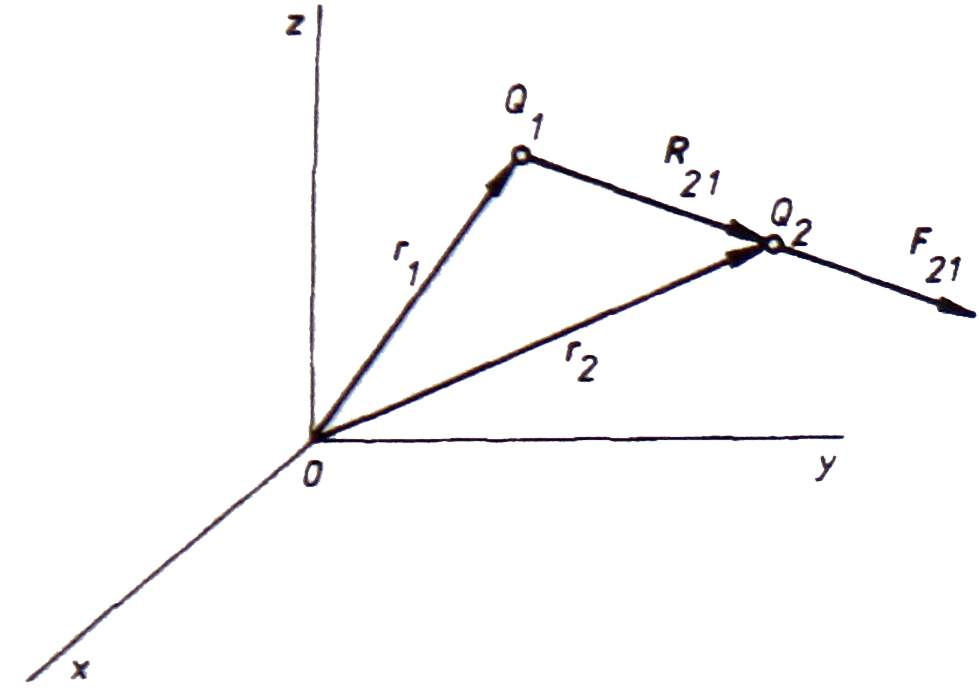
\includegraphics[width=0.8\linewidth]{fyz_fig0342.jpg}
      \caption{K vzájemnému silovému působení dvou bodových nábojů (\cite[s.~294]{Feynman02}).}
      \label{fyz:fig0342}
    \end{figure}

    Sílu působící mezi dvěma malými nabitými kuličkami lze měřit z úhlu zkrutu a dlouhého a tenkého
    vlákna délky \(l\) a poloměru průřezu \(R\). Úhel \(\alpha\) se zjišťuje odrazem světelného
    paprsku od zrcátka \(Z\) spojeného s vláknem. Na konci vlákna je zavěšeno vodorovné vahadélko s
    malými stejnými kuličkami na koncich. Jedna z těchto pohyblivých kuliček nesoucí elektrický
    náboj \(Q_2\) se ustáli v rovnovážné poloze vůči nehybné kuličce o náboji \(Q_1\) ve vzdálenosti
    \(R_{12}\) (obr. \ref{fyz:fig0343}). Jak uvidíme později, nabitá kulička se navenek chová jakoby
    elektrický náboj byl umístěn v jejím středu a popsané uspořádání tedy umožňuje měřit síly
    působící mezi bodovými náboji. Moment \emph{tangenciální síly} \(\vec{F}_t\) se musí rovnat
    \emph{torznímu momentu} \(\vec{D}\) takže platí

    \begin{equation}\label{fyz:eq372}
      rF_t = D = \frac{\pi}{2}\frac{GR^4}{l}\alpha
    \end{equation}
    kde \(r\) je délka ramene torzních vah, \(G\) modul smyku materiálu vlákna), a tedy
    \begin{equation}\label{fyz:eq373}
      F_{21} = \dfrac{F_t}{\cos\dfrac{\alpha}{2}} = \dfrac{D}{r\cos\dfrac{\alpha}{2}}
    \end{equation}
    
    Na základě výsledků těchto experimentů lze formulovat vztah vyjadřující sílu \(\vec{F}_{12}\),
    kterou náboj \(Q_1\) působí na náboj \(Q_2\). Tento vztah, známý jako \textbf{Coulombúv zákon},
    lze napsat ve tvaru
    \begin{equation}\label{fyz:eq374}
      \vec{F}_{21} = k\frac{Q_1Q_2}{R_{21}^3}\vec{R}_{12}
    \end{equation}
    v němž \(\vec{R}_{21} = \vec{r}_2 - \vec{r}_1\) a \(R_{21}\) je velikost vektoru
    \(\vec{R}_{21}\). Obráceně sílu \(\vec{F}_{12}\), kterou působí náboj \(Q_2\) na náboj \(Q_1\),
    dostaneme záměnou indexů \(1\) a \(2\) ve vztahu (\ref{fyz:eq374}). Platí tedy \(\vec{F}_{21} =
    -\vec{F}_{12}\) v souladu s \emph{Newtonovým principem akce a reakce}. Síly mezi bodovými náboji
    působí podél jejich spojnice - takové síly nazýváme \emph{centrálními}. Změní-li se znaménko
    součinu \(Q_1Q_2\), změní se pouze směr síly a nikoli její velikost. Kladné znaménko tohoto
    součinu odpovídá přitom síle odpudivé, záporné znaménko síle přitažlivé. 
      
    \begin{figure}[ht!]  %\ref{fyz:fig0343}
      \centering
      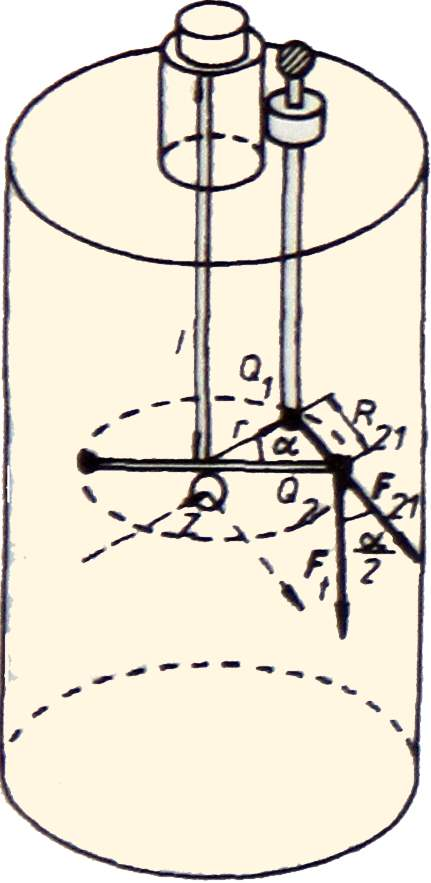
\includegraphics[width=0.5\linewidth]{fyz_fig0343.jpg}
      \caption{Coulombovy torzní váhy (\cite[s.~294]{Feynman02}).}
      \label{fyz:fig0343}
    \end{figure}
    
    Velikost síly působící mezi dvojicí bodových nábojů je rovna
    \begin{equation}\label{fyz:eq375}
      F = \abs{\vec{F}_{21}} = \abs{\vec{F}_{12}} = k\frac{\abs{Q_1Q_2}}{R_{21}^2}
    \end{equation}
    Tato velikost klesá se čtvercem vzdálenosti obou nábojů (stejně jako gravitační působení dvou
    hmotných bodů) a nezávisí na směru v prostoru. Coulombovy síly jsou tedy izotropní.
    
    Všimneme si nyní poněkud obecnější úlohy. Předpokládejme, že v bodech o polohových vektorech
    \(\vec{r}_1, \vec{r}_2, \ldots, \vec{r}_N\) jsou rozloženy bodové náboje \(Q_l, Q_2, \ldots,
    Q_N\). Nechť dále v bodě o polohovém vektoru \(\vec{r}\) je umístěn bodový náboj \(Q\). Ptáme
    se, jaká síla \(\vec{F}\) bude na náboj \(Q\) působit. Abychom na tuto otázku mohli odpovědět,
    musíme vědět, jak se změní silové působení mezi dvojicí bodových nábojů, budou-li v prostoru
    rozmístěny ještě náboje další. 
    
    Experimentální zkušenost ukazuje, že silové působení mezi danou dvojicí nábojů je na přítomnosti
    dalších nábojů nezávislé. Podle \emph{věty o skládání sil}, známé z mechaniky, můžeme proto
    celkovou sílu \(\vec{F}\) působící na náboj \(Q\) vyjádřit jako vektorový součet sil
    \(\vec{F}_i\) (\(i = 1, \ldots,N\)) vyvolaných jednotlivými náboji \(Q_1\) až \(Q_N\). Podle
    (\ref{fyz:eq374}) bude tedy platit
    
  \todo[inline]{Kapitola fyz3ch01 je pahýl}  